\subsubsection[The \xtsvty]{The $\boldsymbol{\xtsvty}$}
\label{sec:x1070}

While searching for potential backgrounds resulting from misidentifying two hadrons as muons, a
peak was found in the $m(\mumu\leftrightarrow\kk)$ spectrum.
This peak was consistent with the \xtsvty listed in the PDG~\cite{PDG2012}, which has a mass of
$(1072\pm1)\mev$ with a width of $(3.5\pm0.5)\mev$ and was observed in the $\KS\KS$ distribution
from $\pim p \to \KS \KS n m\piz$ collisions~\cite{x1070vlad} (for $m\in\mathbb{Z}$).
Figure~\ref{fig:x1070} shows the observation of this resonance from \Ref{x1070vlad} alongside
the data from this analysis.

%\begin{figure}
  %\begin{center}
    %\subfloat[\label{fig:x1070:vlad}]{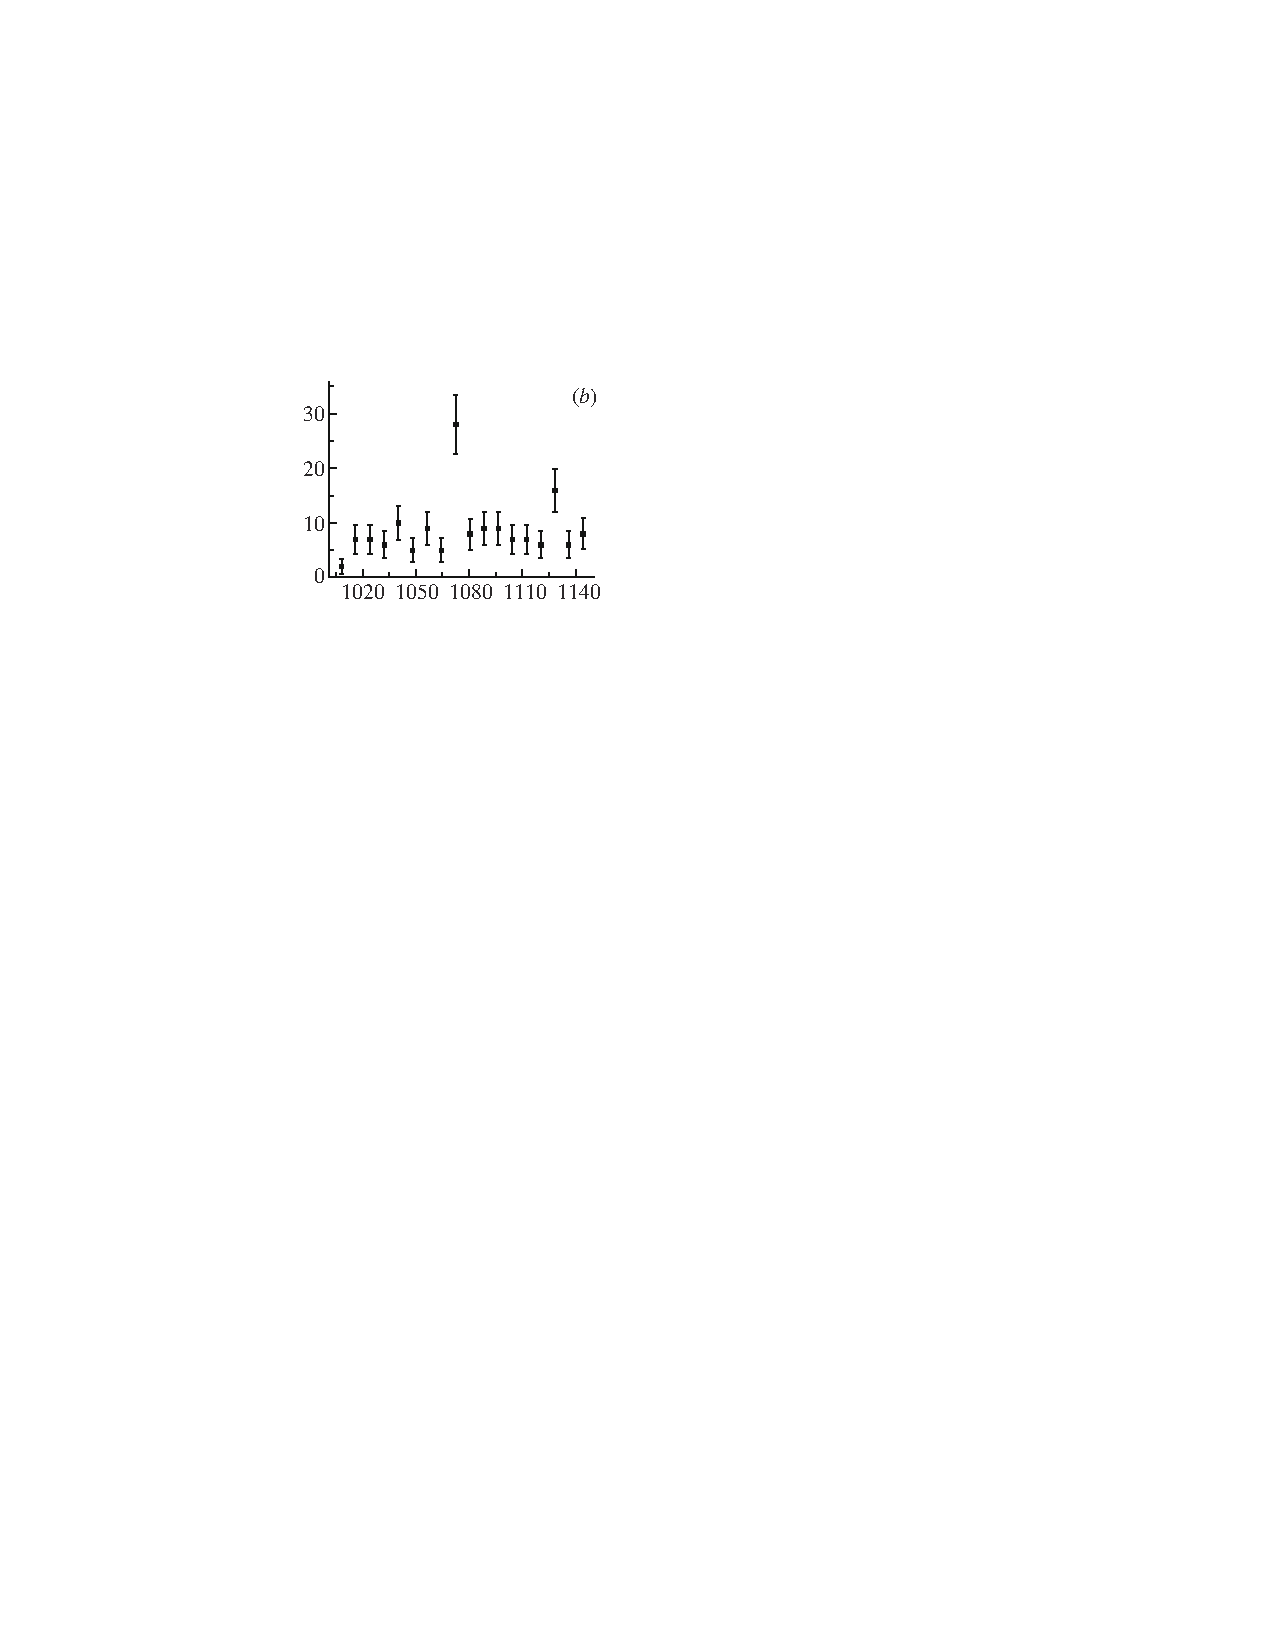
\includegraphics[height=0.2\textheight]{x1070vlad}}
    %\subfloat[\label{fig:x1070:data}]{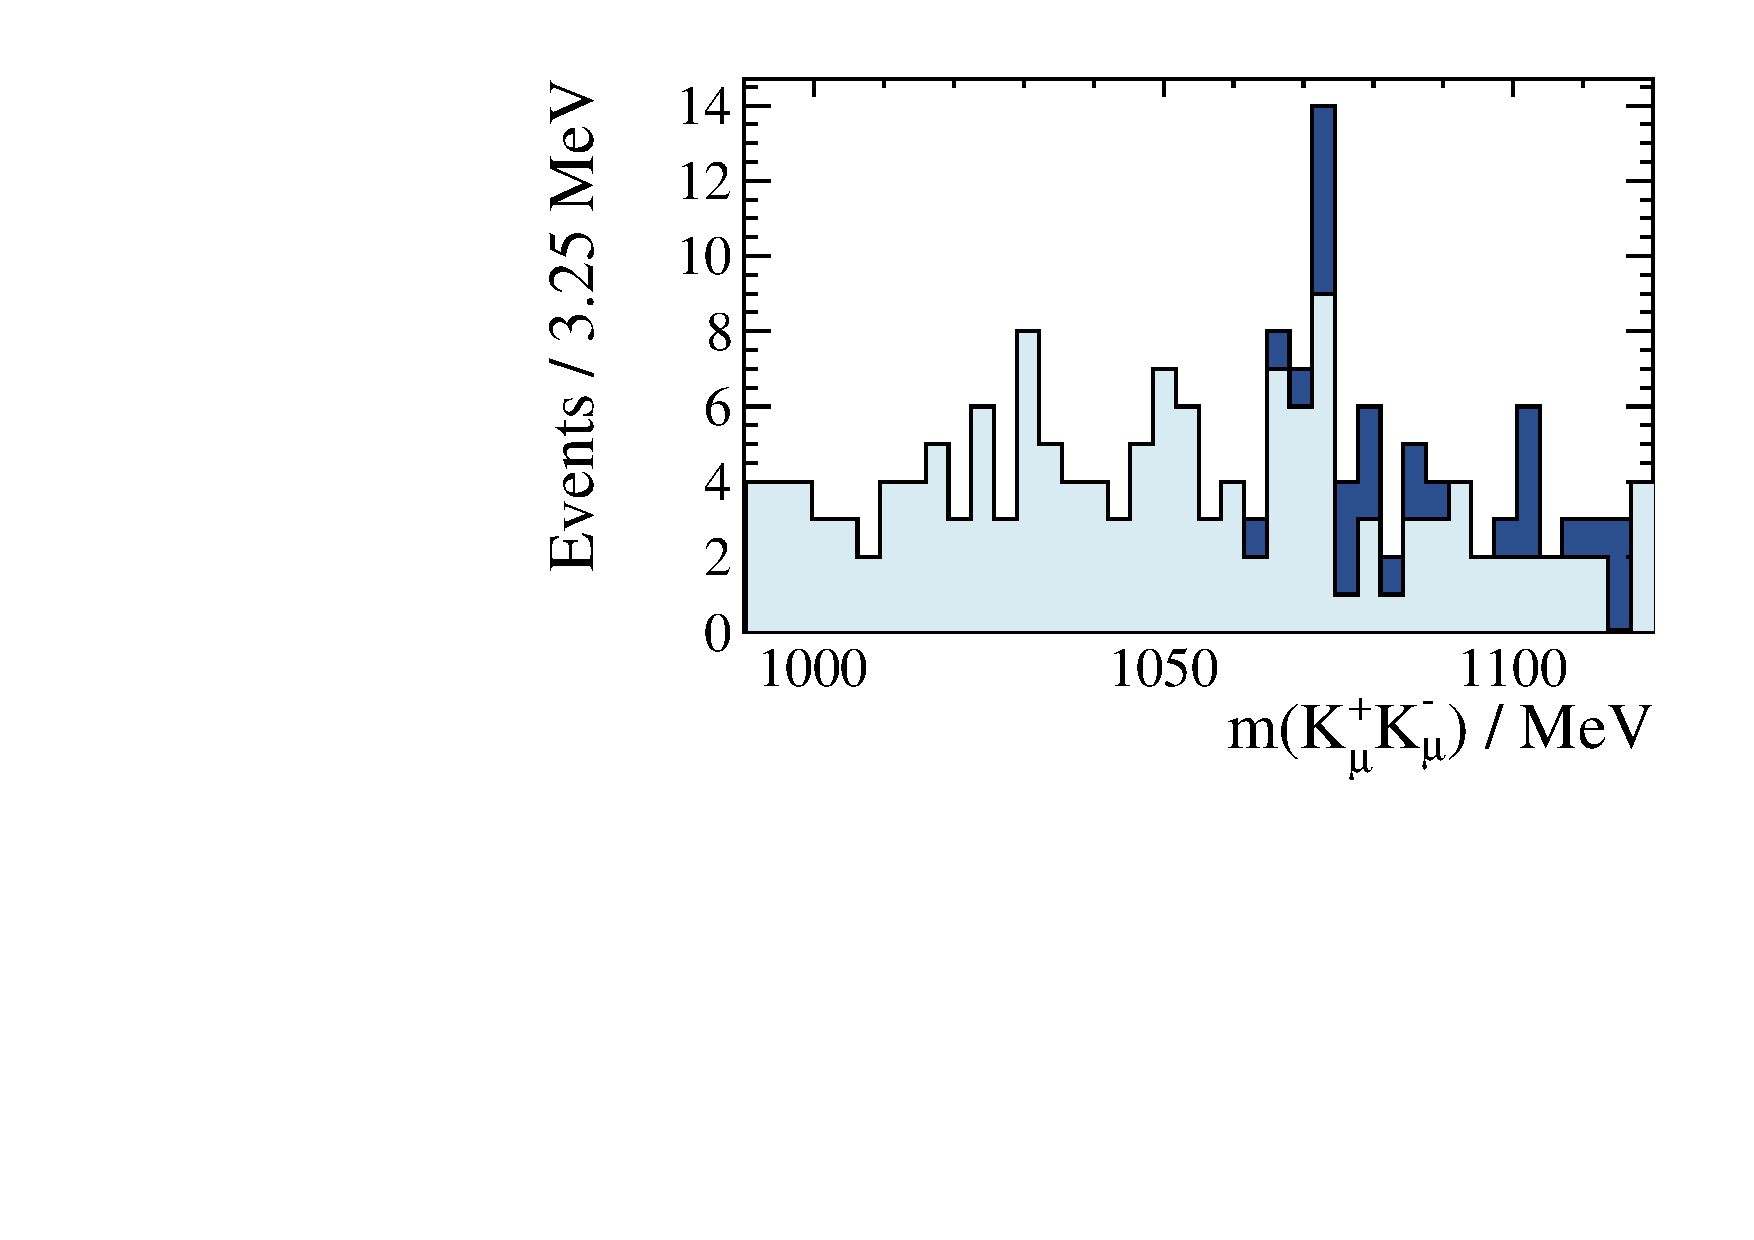
\includegraphics[height=0.2\textheight]{mumu_kk}}
    %\caption{\small
      %A comparison of
      %\protect\subref{fig:x1070:vlad} the data which observes the \xtsvty~\protect\cite{x1070vlad}
      %and
      %\protect\subref{fig:x1070:data} data, where the muons candidates have been assigned the kaon
      %mass.
      %The latter of these plots also shows a dashed line indicating the effect of vetoing
      %\decay{\KS}{\pip\pim}, as described in
      %Sec.~\protect\ref{sec:backgrounds:misid}, and a dotted line showing
      %the effect of removing the entire \KS region.
    %}
    %\label{fig:x1070}
  %\end{center}
%\end{figure}

Figure~\ref{fig:x1070:2d} shows a comparison of simulated \decay{\KS}{\pipi} decays with the observed data near this ``peak''.
It is clear that \decay{\KS}{\pipi} decays produce a peak at 1070\mev under the \kk hypothesis.  There is also a long tail but with low statistics and with a roughly uniform background this tail would not be expected to be visible in the data.

%\begin{figure}
  %\begin{center}
    %\subfloat[\label{fig:x1070:2dphsp}Phasespace simulation]
    %{\includegraphics[width=0.48\textwidth]{anax1070tgen_swap_mumu_kk}}
    %\subfloat[\label{fig:x1070:2ddata}Data]
    %{\includegraphics[width=0.48\textwidth]{anax1070data_2d}}\\
    %\subfloat[\label{fig:x1070:2dphsp:pipi}Projection of $\pipi$ from simulated decays]
    %{\includegraphics[width=0.48\textwidth]{anax1070tgen_pipi}}
    %\subfloat[\label{fig:x1070:2dphsp:kk}Projection of $\kk$ from simulated decays]
    %{\includegraphics[width=0.48\textwidth]{anax1070tgen_kk}}\\
    %\subfloat[\label{fig:x1070:2ddata:pipi}Projection of $\pipi$ from data]
    %{\includegraphics[width=0.48\textwidth]{anax1070data_swap_mumu_pipi}}
    %\subfloat[\label{fig:x1070:2ddata:kk}Projection of $\kk$ from data]
    %{\includegraphics[width=0.48\textwidth]{anax1070data_swap_mumu_kk}}
    %\caption{\small
      %A comparison of \decay{\KS}{\pi\pi} under different mass hypotheses, for
      %\protect\subref{fig:x1070:2dphsp} simulated \decay{\KS}{\pipi} events, and
      %\protect\subref{fig:x1070:2ddata} \decay{\Bd}{\Kstarz\db} data after the stripping.
      %%of \decay{\KS}{\pipi}.
      %The $x$-axis in both cases have the particles assigned the pion mass, and the $y$-axis are
      %the masses working under the \kk mass hypothesis.
      %Projections from of 2D plots are also shown for silmulation:
      %\protect\subref{fig:x1070:2dphsp:pipi} di-pion mass, and
      %\protect\subref{fig:x1070:2dphsp:kk} the \kk mass with the pions under the kaon mass
      %hypothesis;
      %and data:
      %\protect\subref{fig:x1070:2ddata:pipi} $x$-axis with the muons under the pion mass hypothesis,
      %\protect\subref{fig:x1070:2ddata:kk} $y$-axis with the muons under the kaon mass hypothesis.
      %Dotted lines indicate $m(\kk)=1070\mev$.
      %%Here, data is straight out of the stripping.
    %}
    %\label{fig:x1070:2d}
  %\end{center}
%\end{figure}


Applying the \KS vetoes described in \Sec{sec:backgrounds:misid} removes
some of this contribution, but not all of it.
Figure~\ref{fig:x1070:data} shows the distribution of $m(\mumu\leftrightarrow\kk)$ with
the \KS vetoes applied and with the entire \KS region removed ($|m(\mumu\leftrightarrow\pipi)-m(\KS)|<25\mev$); in all
cases there is a contribution at $1070\mev$ above the level of the background.
This is likely due to decay in flight of the pions which causes them to pass the stringent muon identification criteria and to fail the \KS mass veto.
While there is still a small background yield that survives, it does not peak in dimuon mass and so is not a concern.











